% !TeX spellcheck = en_US
\documentclass[preprint,times,sort&compress]{elsarticle}
\usepackage{chemmacros}
\usepackage{chemgreek}
\usepackage{textgreek}
\usepackage{chemschemex}
\usepackage{tikz}
\usepackage{polyglossia}
\usepackage{siunitx}


% TEMPORALES
\usepackage{lineno}

\begin{frontmatter}

    \title{Computational study of the glycolytic degradation of \iupac{poly|(ethylene terephthalate} catalyzed by \iupac{\N^1,\N^2-bis|(2-amino|benzyl)|-1,2-|diamino|ethane zinc(II)}}

    \author[1]{Pablo E. Alanis González\corref{cor1}}
    \cortext[cor1]{Corresponding author}
    \ead{pabloalanis1998@gmail.com}

    \author[1]{Isabel del Carmen Saenz Tavera}

    \author[1]{Victor Manuel Rosas García}

    \affiliation[1]{organization={Facultad de Ciencias Químicas, Universidad Autónoma de Nuevo León},
        addressline={Av. Universidad s/n, Cd. Universitaria},
        city={San Nicolás de los Garza},
        postcode={66455},
        state={Nuevo León},
        country={México}}

    \begin{abstract}
        A possible reaction mechanism of the glycolytic degradation of \iupac{poly|(ethylene terephthalate)} (PET) catalyzed with \iupac{\N^1,\N^2-bis|(2-amino|benzyl)|-1,2-|diamino|ethane zinc(II)} (ABEN) was determined using KS-DFT using the meta-NGA global-hybrid functional, MN15 \cite{Yu2016a} up to def2-SVP/def2-TZVP level of theory making use of an energy-weighted climbing image nudged elastic band (EW-CI-NEB) algorithm \cite{Asgeirsson2021} to determine the minimum energy path (MEP) and then optimizing the converged climbing image (CI) using eigenvector-following partitioned rational function optimization (EF P-RFO) to obtain the transition state (TS). The non-covalent interactions where obtained using and averaged independent gradient model (aIGM) algorithm \cite{Lefebvre2018}
    \end{abstract}

    %%Graphical abstract
    \begin{graphicalabstract}
        %\includegraphics{grabs}
    \end{graphicalabstract}

    %%Research highlights
    \begin{highlights}
        \item Research highlight 1
        \item Research highlight 2
    \end{highlights}

    \begin{keyword}

        %% Keywords
        KS-DFT \sep Polymer degradation \sep Catalysis

        % Codigos PACS
        \PACS 82.20.Pm \sep 82.35.-x \sep 82.65.Jn
    \end{keyword}

\end{frontmatter}

% \author{Pablo E. Alanis González}
% \affiliation[Universidad Autónoma de Nuevo León]
% {Universidad Autónoma de Nuevo León, San Nicolás de los Garza, N.L.}
% \altaffiliation{Facultad de Ciencias Químicas, UANL}
% \email{pabloalanis1998@gmail.com}
% \phone{+52 (81) 1177 3600}

% \author{Isabel del Carmen Saenz Tavera}
% \affiliation[Universidad Autónoma de Nuevo León]
% {Facultad de Ciencias Químicas, Universidad Autónoma de Nuevo León, San Nicolás de los Garza, N.L.}
% \altaffiliation{Facultad de Ciencias Químicas, UANL}

% \author{Victor Manuel Rosas García}
% \affiliation[Universidad Autónoma de Nuevo Leon]
% {Facultad de Ciencias Químicas, Universidad Autónoma de Nuevo León, San Nicolás de los Garza, N.L.}
% \altaffiliation{Facultad de Ciencias Químicas, UANL}

%%%%%%%%%%%%%%%%%%%%%%%%%%%%%%%%%%%%%%%%%%%%%%%%%%%%%%%%%%%%%%%%%%%%%
%% The document title should be given as usual. Some journals require
%% a running title from the author: this should be supplied as an
%% optional argument to \title.
%%%%%%%%%%%%%%%%%%%%%%%%%%%%%%%%%%%%%%%%%%%%%%%%%%%%%%%%%%%%%%%%%%%%%

% \title{Computational study of the glycolytic degradation of \iupac{poly|(ethylene terephthalate)} catalyzed by \iupac{\N^1,\N^2-bis|(2-amino|benzyl)|-1,2-|diamino|ethane zinc(II)}}

%%%%%%%%%%%%%%%%%%%%%%%%%%%%%%%%%%%%%%%%%%%%%%%%%%%%%%%%%%%%%%%%%%%%%
%% Some journals require a list of abbreviations or keywords to be
%% supplied. These should be set up here, and will be printed after
%% the title and author information, if needed.
%%%%%%%%%%%%%%%%%%%%%%%%%%%%%%%%%%%%%%%%%%%%%%%%%%%%%%%%%%%%%%%%%%%%%
% \abbreviations{DFT,meta-NGA,PET,ABEN,EG}
% \keywords{Depolimerization,PET,Zinc catalists}

% \begin{document}

% \abstract{
% \linenumbers
% A possible reaction mechanism of the glycolytic degradation of \iupac{poly|(ethylene terephthalate)} (PET) catalyzed with \iupac{\N^1,\N^2-bis|(2-amino|benzyl)|-1,2-|diamino|ethane zinc(II)} (ABEN) was determined using KS-DFT using the meta-NGA global-hybrid functional, MN15 \cite{Yu2016a} up to def2-SVP/def2-TZVP level of theory making use of an energy-weighted climbing image nudged elastic band (EW-CI-NEB) algorithm \cite{Asgeirsson2021} to determine the minimum energy path (MEP) and then optimizing the converged climbing image (CI) using eigenvector-following partitioned rational function optimization (EF P-RFO) to obtain the transition state (TS). The non-covalent interactions where obtained using and averaged independent gradient model (aIGM) algorithm \cite{Lefebvre2018}

\section{Introduction}

By 2015, the annual global production of plastics surpassed 367 million tonnes; \SI{55}{\percent} of all plastic waste was discarded, \SI{25.5}{\percent} incinerated and just \SI{19.5}{\percent} was recycled \cite{Geyer2017}. \iupac{Poly|(ethylene terephthalate)} (PET) is one of the most widely traded polymer there is on the market. It is mainly used in the fabrication of bottles, packages and fibers. The widespread usage of this plastic is due to its properties, like an excellent tensile strength, chemical resistance, clarity, processability and a reasonable thermal stability. It is also very cheap to produce \cite{Caldicott1999,Thompson2009}. Albeit all its properties, PET is also becoming a global problem, since a lot of it is not recycled at all. It is becoming a waste problem. Even tough PET by itself is not harmful to humans and by itself does not impose an environmental damage, because of its substantial presence in bodies of water and its high resistance to biological and atmospheric agents, PET is classified as a nocive material \cite{Paszun1997}.
Chemical recycling of PET has become an important topic since this is the most sustainable way of recycling plastic, and produces \latin{de novo} the starting materials of the synthesis of PET. There is an extensive amount of literature on the topic of chemical degradation of PET, processes such as methanolysis, hydrolysis and glycolysis have been thoroughly  studied \cite{Campanelli1993,Campanelli1994,Campanelli1994a}. The most sustainable reaction of degradation of PET is the glycolysis since this reaction produces \iupac{bis|(2-hidroxy|ethyl) terephthalate} (BHET), one of the precursors of PET itself. PET glycolysis, nevertheless is not a very effective process if no catalyst is used. Plenty of studies have been made on the reaction of the degradation of PET via catalyzed glycolysis. Some transition metals such as zinc lead to a good yield in this type of reactions with the benefit that zinc is not a very toxic metal.
For the chemical recycling of PET, numerous protocols involving hydrolysis, methanolysis and glycolysis among many others \cite{Campanelli1993,Campanelli1994,Campanelli1994a} have been reported. The uncatalyzed glycolysis of PET is not an effective process; transition metal (TM) salts have been determined to aid in this reaction. The oldest report of the catalyzed glycolytic degradation of PET was reported by \citet{Vaidya1988} in which they carried the reaction using different metal acetates as catalysts. Then it was determined that \ch{Zn^{II}} has a greater catalytic activity in the glycolysis than other TM (\ch{Mn^{II}}, \ch{Co^{II}} and \ch{Pb^{II}}) \cite{Ghaemy2005}. Alongside the numerous zinc catalysts studied to date, a novel zinc catalyst, \iupac{\N^1,\N^2-bis|(2-amino|benzyl)|-1,2-|diamino|ethane zinc(II)} (ABEN) \cite{Elizondo-Martinez2013} has shown to have a great catalytic activity \ref{Sc1} in the glycolytic degradation of PET yielding around \SI{78}{\percent} of BHET\cite{Ovalle-Sanchez2017}. The main purpose of this article is to evaluate the possible reaction mechanism involved in this catalyzed glycolytic depolymerization of PET with ABEN and determine the covalent or non-covalent interactions involved.\cite{Abdelaal2008,Nikje2006}
%PRUEBA
\begin{scheme}
    \centering
    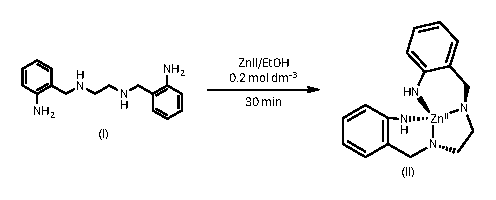
\includegraphics[width=0.85\linewidth]{figures/Synth_ABEN.eps}
    \caption{Reported synthesis of ABEN \cite{Elizondo-Martinez2013}. The structure of ABEN (II) was derived from the electronic structure computations obtained in this study.}
    \label{Sc1}
\end{scheme}

\section{Methods}

The starting configurations for EG and ABEN where proposed and optimized using XTB \cite{Bannwarth2021} with the force field GFN2-xTB \cite{Bannwarth2019}. The staring configuration for DBHET was proposed using crystallographic data \cite{Daubeny1954}, then reoptimized using $r^2\textrm{SCAN-3c}\textrm{def2/SVP}$. The final point energies where obtained all obtained using \chemomega-B97X-D4/def2-SVP and def2-TZVPP on just the oxygen, nitrogen, and  zinc atoms.
The optimized structures where then merged onto the same Cartesian coordinates and then re-optimized in $r^2\textrm{SCAN-3c}\textrm{def2/SVP}$. Then, a multidimensional relaxed surface scan was performed keeping constrained, and varying the bond distances in 20 steps to obtain the products of the reactions depicted in . The optimized product and the starting geometry of the relaxed surface scan where the input for an Energy-Weighted Climbing image Nudged Elastic Band (EW-CI-NEB) \cite{Asgeirsson2021} algorithm to find the path of minimum energy connecting both ends, followed by a P-RFO optimization to find a TS performed onto the climbing image (CI).

In order to determine covalent and non-covalent interactions regions between the molecules, an analysis based on Hirshfeld partition of molecular density (IGMH) algorithm within multiwfn was performed \cite{Lu2021} onto the optimized reactant. To minimize computation time, aIGM was performed with the MEP obtained by NEB-TS.

With JANPA \cite{Nikolaienko2014}, CLPOs and bond orders for the reactants, products and transition states where obtained.

% \bibliography{PEAG-ref}

%% Loading bibliography style file
%\bibliographystyle{model1-num-names}
\bibliographystyle{cas-model2-names}

% Loading bibliography database
\bibliography{PEAG-ref}

\end{document}